\documentclass[10pt, a4paper]{article}
\usepackage{geometry}
\usepackage{listings}
\usepackage{hyperref}
\usepackage{graphicx}
\usepackage{ragged2e}
\usepackage{color}
\usepackage{xepersian}
\usepackage{subfiles}
\newgeometry{left=2.4cm, right=2.4cm, bottom=2.4cm}
\settextfont[Scale=1]{XB Roya}
\usepackage{multirow}
\renewcommand{\baselinestretch}{1.5}

\begin{document}
\centerline{گزارش بررسی پیکربندی نامناسب سرویس‌های NoSQL در اشل پروژه‌های بزرگ
به تفکیک تکنولوژی‌های NoSQL}
\centerline{علیرضا سلطانی نشان}
\centerline{\today}
\tableofcontents

\newpage

\section{تعریف مسئله}

ذخیره‌سازی اطلاعات از مهم‌ترین نیاز‌های تحلیل کنندگان داده است. امروزه با توجه
به پیشرفت صنعت IoT و یادگیری ماشین، تولید داده‌ها بسیار افزایش یافته است به
گونه‌ای که بتوان این داده‌ها را به سریع‌ترین روش ممکن در محلی مناسب ذخیره‌سازی و
نگهداری کرد.  افراد برای ذخیره‌سازی این داده‌ها نیاز به نصب و راه‌اندازی یک
سیستم DBM دارند که از طریق یک واسط با زبانی مناسب بتوانند به آن متصل شده و
داده‌های دریافتی را بعد از تجزیه و تحلیل آنها در این محل ذخیره‌سازی و مدیریت
کنند. امروزه محققان ترجیح می‌دهند به دلیل مقیاس پذیری بیشتر، سیستم‌های توزیع شده
و قابلیت پایداری بالا از دیتابیس‌های رابطه‌ای به سمت دیتابیس‌های NoSQL مهاجرت
کنند.  این نوع دیتابیس‌ها امروزه توسط تمام اپلیکیشن‌های جدید پشتیبانی می‌شوند و
برای استفاده آسان طراحی شده‌اند. حتی می‌توان متذکر شد که تعداد زیادی از
سرویس‌های ذخیره‌سازی ابری امروزه‌ از سرویس‌های دیتابیسی NoSQL پشتیبانی گسترده‌ای
دارند. این ارائه دهندگان اغلب شرکت‌های معروفی مانند \lr{Amazon DynamoDB}
\lr{Google Cloud Database} \lr{MS Azure CosmosDB} می‌باشند. همچنین بیشتر این
موتور‌های دیتابیسی به صورت متن‌باز هستند و توسعه دهندگان زیادی از سرتاسر جهان
روی آنها مشغول توسعه هستند.

در سال‌های اخیر، با پدید آمدن و رشد سریع سرویس‌های دیتابیسی NoSQL بین عموم
توسعه‌دهندگان استفاده از این نوع سرویس‌ها افزایش یافته است. دلیل اصلی این
محبوبیت نصب و راه‌اندازی و استقرار آسان آنها در هر محلی است. همچنین قابل اعتماد
هستند، روش‌ها و مکانیزم‌های زیادی برای تهیه نسخه‌های پشتیبان‌گیر به صورت منظم از
داده‌ها را ارائه می‌دهند. دلیل اصلی آسان بود این سیستم آن است که در هنگام
راه‌اندازی آنها زمان زیادی را صرف نمی‌کنید، زیرا بعد از نصب اولیه و طی کردن
فرایند نصب با زدن روی دکمه "بعدی" دیتابیس شما آمادست و می‌توانید از آن در برنامه
خود استفاده کنید. بعد از این فرایند هیچ عملیاتی بر روی تعریف دسترسی‌ها، مدیریت
کاربران در استفاده از دیتابیس مانند اختصاص سطح دسترسی، توسط راه‌انداز سیستم DBM
صورت نمی‌گیرد. نتیجه این موارد پیکربندی غیر اصولی و اشتباه
\footnote{Misconfigured} سیستم ذخیره‌سازی داده می‌شود که در نتیجه افشای اطلاعات
حساس \footnote{\lr{Data Leakage}} را به دنبال خواهد داشت.

سوالی که ممکن است در اینجا مطرح شود آن است که چه زمانی پیکربندی نادرست موجب
افشای اطلاعات می‌شود؟

در ابتدا بعد از راه‌اندازی این نوع دیتابیس‌ها اولین هدف استفاده از آنها در محیط
لوکال در یک شبکه است. اما افشای اطلاعات و پیکربندی اشتباه زمانی رخ می‌دهد که این
دیتابیس‌ها در شبکه اینترنت مورد دسترسی قرار گیرند.

محققان با توجه به موارد گفته شده بالا توانسته‌اند یک ابزار خودکار جهت آنالیز و
جست و جوی سیستم‌های دیتابیسی NoSQL را توسعه دهند که به وسیله آن می‌توانند
پیکربندی نامناسب این سیستم‌های مستقر شده را متوجه شده، موارد آسیب‌پذیری را گزارش
و سپس به صاحبان این دیتابیس‌ها هشداری در جهت در خطر بودن اطلاعاتشان ارسال کنند.

در این گزارش به طور خلاصه تمام موارد انجام شده را در پنج عنوان توضیح می‌دهیم. در
ابتدا در مورد چالش‌ها و نحوه تحقیق روی این آسیب پذیری‌ها و عدم وجود پیکربندی
مناسب می‌پردازیم. در بخش مدل پیشنهادی بیشتر ماهیت ابزار توسعه داده شده را مطرح
می‌کنیم و سپس نتایج اجرای این ابزار را نمایش می‌دهیم و در نهایت به نوآوری و
کار‌های آینده می‌پردازیم.

\newpage

\section{چالش‌ها}

ابزاری توسعه داده شده است که در یک رنج گسترده‌ای از آدرس‌های IP می‌تواند اینگونه
دیتابیس‌ها را اسکن کند و افشای سرویس آنها را تشخیص دهد. این تشخیص به شکل ایمن
بدون هیچ نگهداری داده‌ها و یا افشای اطلاعات حساس آنها صورت می‌گیرد. بررسی ضعف
پیکربندی‌های صورت گرفته بر روی ۶۷ میلیون ۷۲۶ هزار و ۶۴۱ آدرس IP بوده است که بین
بازه زمانی اکتبر ۲۰۱۹ و مارچ ۲۰۲۰ تکمیل شده است. نکته جالب از آنجایی شروع می‌شود
که این سرویس‌ها نه تنها به صورت شخصی راه‌اندازی شده‌اند بلکه تعداد ۱۲ هزار و ۲۷۶
نمونه از آنها در ارائه دهندگان سرویس‌های ابری معروف یافت شده است.  با توجه به
این موضوع در این تحقیق ۷۴۲ مورد آسیب پذیری پیدا شده است که به صورت مستقیم وب
سایت این کاربران به دلیل ضعف در پیکربندی به دیتابیس‌های آنها ارجاع دارد این بدان
معناست با وجود تنظیمات و پیکربندی پیش فرض و بدون هیچ گونه استراتژی امنیتی، هر
کاربر ناشناس دیگری می‌تواند وارد این دیتابیس‌ها شده و آنها را با نظر و سلیقه
خودش تغییر و حتی تخریب به قصد اخاذی کند.

\subsection{بررسی نمونه‌ها در پیکربندی ضعیف راه‌اندازی}

\begin{enumerate}
    \item در مارچ ۲۰۲۰، ۷ ترابایت از داده‌های سایت بزرگسالان به صورت صریح از یک
    نمونه دیتابیس \lr{Elastic Search} با اطلاعاتی از قبیل، نام کاربران، جنسیت و
    گرایش‌ها، لاگ‌های مربوط به پرداخت‌هایشان، ایمیل، با ۱۰۸۸ میلیارد رکورد مورد
    افشا قرار گرفت.
    \item در نوامبر سال ۲۰۱۹ یک محقق توانست یک نمونه با پورت باز با بیشتر از ۱/۲
    میلیارد رکورد از یک دیتابیس را پیدا کند که شامل اطلاعات حساس کاربران از قبیل
    آدرس ایمیل آنها بود.
    \item در ژانویه سال ۲۰۱۷، در یک حمله بیشتر از ۶۰۰ نمونه از دیتابیس
    \lr{Elastic search} حذف شدند و برای بازیابی آنها از صاحبانشان اخاذی کردند [۴۰].
    \item براساس گزارشی در سال ۲۰۱۸ بیشتر از ده ها هزار نمونه از دیتابیس‌های
    Redis در دسترس کاربران مخرب، آسیب‌پذیر شناخته شدند که به دلیل دسترسی عموم
    افراد تعداد ۷۵۰۰ سرور یافت شد که در معرض خطر یک بدافزار به نام Botnet بودند
    که هدف اصلی آنها دزدیدن ارز‌های دیجیتال \footnote{Cryptocurrencies} آن
    پلتفرم ارائه دهنده بود.
\end{enumerate}

براساس موارد مطرح شده در بند‌های گفته شده بالا، اولین بررسی از ضعف پیکربندی
دیتابیس‌های NoSQL انجام شده است به گونه‌ای که می‌توان از آن برای تشخیص و تعیین
معیاری برای بررسی پیکربندی درست در این دیتابیس‌ها از آن استفاده کرد. محققان یک
فریمورکی توسعه داده‌اند که به صورت کاملا خودکار می‌تواند سرویس‌های معرض دید عموم
را تشخیص و عملیات بررسی امنیتی روی آنها انجام دهد بدون ذخیره‌سازی داده‌های
کاربران یا باز کردن داده‌های دیتابیس پلتفرم‌ها و دریافت اطلاعات حساس آنها.

\subsection{فرایند کلی عملکرد فریمورک} 

این فریمورک در ابتدا لیستی از آدرس‌های IP که توسط بیشتر ارائه دهندگان سرویس‌های
ابری استفاده می‌شود را اسکن کرده و به دنبال ارتباطی باز بر روی پورت پیش فرض
دیتابیس NoSQL می‌گردد که بتواند به آن به صورت مستقیم متصل شود. (در شکل ۱،
می‌توانید عملکرد فریمورک را در تصویر مشاهده کنید.) سپس می‌تواند به یک نمونه از
دیتابیس دسترسی داشته و عملیات بررسی امنیتی خود را شروع کند.  به طور کلی این
فریمورک به بررسی سطح دسترسی دیتابیس (همان دسترسی‌های خواندن و نوشتن روی یک سیستم
مدیریت دیتابیس) متا دیتا از قبیل نسخه مورد استفاده از سرویس ،NoSQL کاربران مجاز
دسترسی به دیتابیس، سطوح دسترسی تعریف شده و جداول مرتبط به این دیتابیس‌ها،
می‌پردازد. 

\begin{figure}
    \centering
    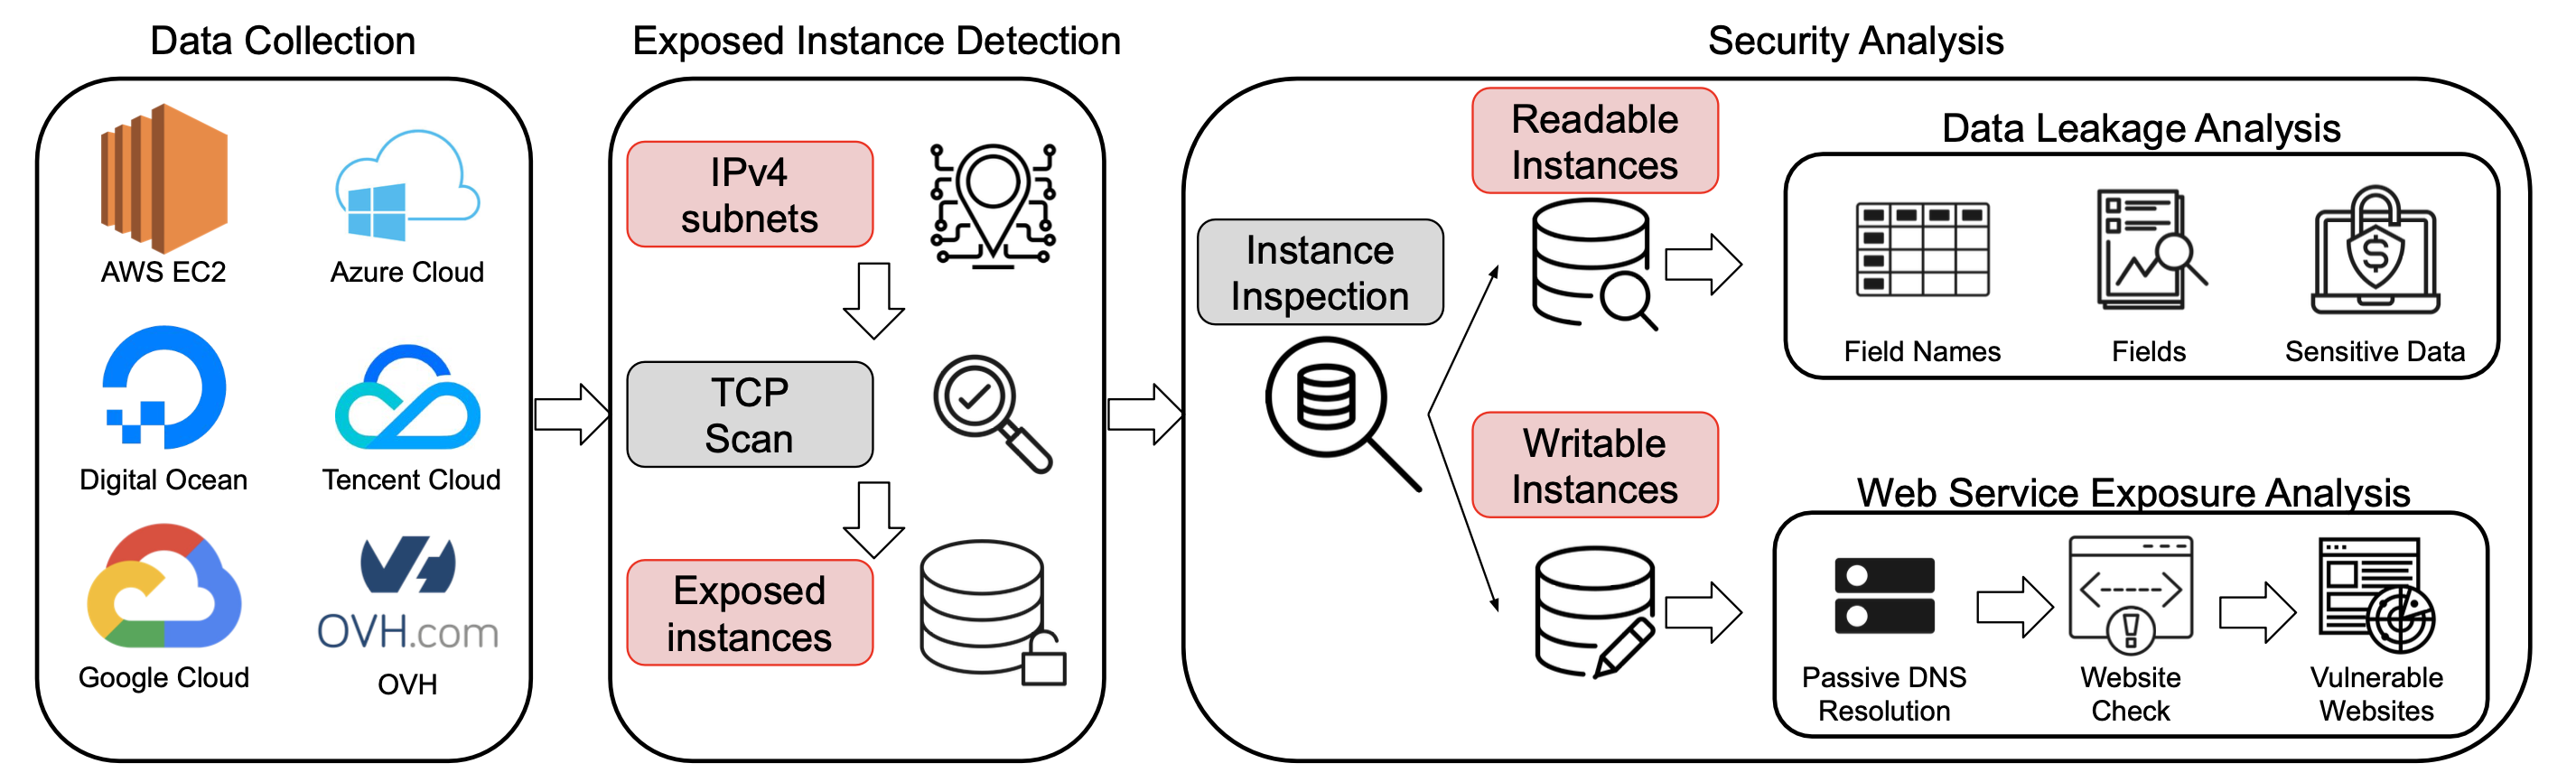
\includegraphics[width=1\textwidth]{res/fig1.png}
    \caption{بررسی عملکرد ابزار توسعه داده شده}
    \label{fig: diagram}
\end{figure}

\subsubsection{تشخیص عمل خواندن از دیتابیس‌های فاش شده}

اگر این ابزار تشخیص دهد که دسترسی خواندن را از این دیتابیس‌ها دارد تضمین افشای
اطلاعات این سیستم‌ها را به طور قطعی می‌دهد که می‌تواند خطری برای محتوای داخل
دیتابیس باشد. ابزاری که توسعه داده شده است کاملا ایمن می‌باشد چرا که اصلا وارد
محتوای این دیتابیس‌ها و داده‌های آنها نشده و تنها از توابعی مانند تابع Count
برای شمارش رکورد‌هایی که مربوط به فیلد‌هایی مانند نام کاربران، شماره تلفن یا
آدرس ایمیل آنها می‌شود، استفاده می‌کند. اغلب داده‌های جمع‌آوری شده از این
دیتابیس‌ها به صورت نمایش تعداد رکورد‌های آنها مربوط به فیلدی مشخص است که در
جداول صفحات بعدی آنها را مشاهده خواهید کرد.

\subsubsection{تشخیص عمل نوشتن از دیتابیس‌های فاش شده}

زمانی که این ابزار بتواند به این دیتابیس‌ها متصل شود و بعد از آن قادر به ساخت یک
workspace یا یک رکوردی از داده‌ NoSQL یعنی همان Document باشد، تشخیص می‌دهد که
مجوز نوشتن را در این سیستم دارد به همین خاطر یک پیام جدی را برای صاحبان دیتابیس
می‌نویسد تا در جریان ضعف پیکربندی و ایمن نبودن ارتباطات آنها و باز بودن
دسترسی‌ها، قرار بگیرند. با این کار محققان از افشا و آسیب به نمونه از دیتابیس
جلوگیری می‌کنند. داشتن دسترسی نوشتن یکی از خطرناک‌ترین دسترسی‌های این دیتابیس‌ها
می‌باشد به طوری که این ابزار علاوه عملیات گفته شده بالا یک استراتژی دیگری را در
پیش می‌گیرد و آن این است که به جست و جوی DNS های آن به صورت غیر فعال می‌پردازد
تا متوجه آن شود که آیا روی این IP که دیتابیس مستقر شده است، منابع دیگری مانند
برنامه‌های وب و وبسایت‌ها و دیگر سرویس‌ها مستقر شده‌اند یا خیر؟ چرا که اگر منابع
وب را از این طریق پیدا کند به این معنی است که این سرور‌ها پتانسیل حمله
آسیب‌زننده‌ای که باعث دستکاری داده‌ها می‌شود را دارند. در تمام وضعیت گفته شده
بالا با ارائه دهندگان سرویس‌های ابری ارتباط برقرار شده و به آنها در مورد
آسیب‌پذیری‌های یافت شده گزارشی به عمل آمده است.

۶۷ میلیون آدرس IP اسکن شده در ارائه دهندگان سرویس‌های ابری مختلف بین اکتبر سال
۲۰۱۹ تا مارچ ۲۰۲۰، تعداد ۱۲,۲۷۶ سرویس دیتابیسی با دسترسی‌های مختلف یافت شدند که
۸۷٪ آنها با دسترسی آزاد خواندن و نوشتن و ۸/۶٪ آنها تنها قابلیت خواندن اطلاعات را
داشتند. بین این بررسی محققان مواردی از قابل دسترس بودن اطلاعات فقط خواندنی این
دیتابیس‌ها پیدا کردند که ۷۴۲ نمونه پتناسیل افشای اطلاعات حساس کاربران مانند آدرس
ایمیل، نام‌ها، گذرواژه‌ها و تمام منابعی که می‌تواند در اپلیکیشن‌های وب آنها
استفاده شود، را داشتند. علاوه‌بر این ما دیتابیس‌های مختلفی را پیدا کردیم که
توانایی افشای فایل‌های مهم و حساس مانند فایل‌های سرتیفیکیت سایت‌ها و لاگ‌های
مربوط به آنها را داشتند. بین تمام سیستم‌های DBM سرویس MongoDB بیشترین مقدار ضعف
پیکربندی را داشت به گونه‌ای که ۴،۸۵۹ نمونه از آن یافت شد و این سهم برای دیتابیس‌
Elasticsearch به مقدار ۴،۷۲۵ نمونه بود.

\subsubsection{مرور سناریو‌های تهدیدآمیز}

\subsubsection*{افشای اطلاعات (سطح دسترسی خواندن)}

زمانی که منابع دیتابیسی به صورت غیر عامدانه‌ای مورد دسترسی عموم قرار می‌گیرد که
موجب مسائل شکسته شدن حریم خصوصی کاربران و افشای اطلاعات حساس و عدم محرمانگی
می‌شود.

\subsubsection*{آلوده شدن منابع وب (سطح دسترسی نوشتن)}

زمانی که دسترسی نوشتن روی یک میزبان فعال باشد به معنای آن است که تمام محتوای آن
میزبان را می‌توان دستکاری کرد. اغلب وب سایت‌ها به این ترتیب تغییر چهره روی آنها
اعمال می‌شود که مربوط به عملیات دستکاری Deface کردن این پایگاه‌های اطلاعاتی است.
همچنین این عمل باعث تاثیر روی محتوای این وب‌سایت‌ها خواهد شد چرا که می‌توانند
وارد دیتابیس شده و اطلاعات مروبطه را دستکاری کنند و به نفع خودشان ویرایشی انجام
دهند. همچنین آسیب‌پذیری‌های دیگر نیز می‌تواند رخ دهد. برای مثال بعد از دسترسی
نوشتن روی این میزبان‌ها می‌توانند از طریق وب‌سایت یک فایل مخرب و آلوده را قرار
داده و کاربران آن را به عنوان فایل مورد نظر بارگیری کرده و باعث آلوده شدن دستگاه
کاربران نهایی شود.

\subsubsection{اخاذی در ازای اطلاعات}

مهاجمان می‌توانند با داشتن دسترسی نوشتن روی این دیتابیس‌ها حمله‌ای انجام دهند که
موجب اخاذی از صاحبان اطلاعات شود. معمولا استراتژی مهاجمان در این خصوص از بین
بردن اطلاعات یا رمزنگاری‌ آنها می‌باشد که در ازای اخاذی از صاحبان دیتابیس یا
داده می‌توانند داده‌ها را به آنها برگردانند یا آنها کلید رمزنگاری آن داده‌ها را
تحویل دهند.

محققان چهار تا از محبوب‌‌ترین دیتابیس‌های NoSQL را مورد بررسی قرار دادند تا نشان
دهند که تحقیقات آنها کافی بوده و تقریبا مهم‌ترین سرویس‌های NoSQL را پوشش داده
است. محققان تحقیقاتی را نسبت به محبوب‌ترین سیستم‌های دیتابیسی براساس وب سایت
\href{https://db-engines.com/en/ranking}{db-engines.com} به عمل آوردند. مهم‌ترین
سوال آن است که چگونه یک سیستم به عنوان محبوب‌ترین سیستم دیتابیسی انتخاب می‌شود؟

انتخاب این دیتابیس‌ها براساس درصد استفاده آنها در وبسایت‌ها، بحث و گفت و گو‌های
گروه‌های فنی، پیشنهادات شغلی در رابطه با متخصص مربوط به این دیتابیس‌ها و
ارتباطشان در شبکه‌های اجتماعی می‌باشد. براساس جدول ۱، رنک دیتابیس‌های مختلف
براساس سایت db-engines آمده است. لازم به ذکر است که این جدول نسبت به جدول داخل
مقاله به روز شده که طی ۳ سال گذشته دیتابیس‌های Redis و Elasticsearch به ترتیب
مقال ۶ و ۷ را بدست آوردند. در حالی که بین سال ۲۰۱۹ تا ۲۰۲۰ مقام Redis و
Elasticsearch به ترتیب ۷ و ۸ بود.

\subsubsection{اهداف تحقیق}

اهداف این تحقیقات به شرح زیر می‌باشد:

 \begin{enumerate}
    \item نتیجه عدم تدابیر امنیتی
    \item بررسی تاثیر ضعف پیکربندی
    \item افزایش آگاهی برای جلوگیری از فاش شدن و دستکاری اطلاعات
 \end{enumerate}

همچنین در بخش‌های بعدی در مورد آگاهی از نگرانی‌های اخلاقی مطرح شده است که در آن
به جمع‌آوری داده‌‌های نتیجه این آزمایشات صرفا برای بررسی محاسبات محققان نسبت به
آسیب‌پذیری داده‌ها در آینده است.

\begin{LTR}
    \begin{table}[h]
        \centering
        \begin{RTL}
            \caption{رنکینگ موتور‌های دیتابیس: ۱۰ دیتابیس محبوب از نظر سایت db-engines}
        \end{RTL}
        \scalebox{0.7}{
            \begin{tabular}{c|c|c|c|c|c|c|c}
            \multicolumn{3}{c|}{\textbf{رنک}} & {\textbf{دیتابیس‌}} & {\textbf{مدل}} & \multicolumn{3}{c}{\textbf{امتیاز}} \\
            \hline
                \textbf{نوامبر ۲۰۲۳} & \textbf{اکتبر ۲۰۲۳} & \textbf{نوامبر ۲۰۲۲} & & & \textbf{نوامبر ۲۰۲۳} & \textbf{اکتبر ۲۰۲۳} & \textbf{نوامبر ۲۰۲۲} \\
                1  & 1  & 1 & Oracle & R & $1277.03$ & \textcolor{green}{$+15.61$} & \textcolor{green}{$+35.34$}  \\
                2  & 2  & 2 & MySQL & R & $1115.24$ & \textcolor{red}{$-18.07$} & \textcolor{red}{$-90.30$} \\
                3  & 3  & 3 & MSSQL Server & R & $911.42$ & \textcolor{green}{$+14.54$} & \textcolor{red}{$-1.09$} \\
                4  & 4  & 4 & PostgreSQL & R & $636.86$ & \textcolor{red}{$-1.96$} & \textcolor{green}{$+13.70$} \\
                5  & 5  & 5 & MongoDB & NS & $428.55$ & \textcolor{red}{$-2.87$} & \textcolor{red}{$-49.35$} \\
                6  & 6  & 6 & Redis & NS & $160.02$ & \textcolor{red}{$-2.95$} & \textcolor{red}{$-22.03$} \\
                7  & 7  & 7 & Elasticsearch & NS & $139.62$ & \textcolor{green}{$+2.48$} & \textcolor{red}{$-10.70$} \\
                8  & 8  & 8 & IBM Db2 & R & $139.62$ & \textcolor{green}{$+2.48$} & \textcolor{red}{$-10.70$} \\
                9  & 9  & 10 & SQLite & R & $124.58$ & \textcolor{green}{$+1.13$} & \textcolor{red}{$-13.56$} \\
                10  & 10  & 9 & Microsoft Access & R & $124.49$ & \textcolor{green}{$+0.18$} & \textcolor{red}{$-10.53$} \\
                \hline
            \end{tabular}
        }
    \end{table}
\end{LTR}

\section{مدل پیشنهادی}

\subsection{جمع‌آوری داده با پیدا کردن آدرس‌های IP سرویس دهندگان}

اولین مرحله از این رویکرد جمع‌آوری داده با استفاده از لیست آدرس‌های IP نسخه ۴
بوده است که می‌تواند امکان داشته باشد روی هر کدام از آدرس‌ها حداقل یک نمونه
دیتابیس NoSQL وجود داشته باشد. همچنین محققان لیستی از ارائه دهندگان سرویس‌های
ابری را مطرح کردند که در آنها امکان نصب و راه‌اندازی این نوع دیتابیس‌ها میسر
بوده است. این ارائه دهندگان به کاربران اجازه می‌دهند تا سرویس‌های دیتابیسی خود
را در شبکه اینترنت مستقر کنند و یک \lr{Connection String} معتبر برای دسترسی آنها
به اپلیکیشن‌ خود راه‌اندازی نمایند.

این سرویس‌ها عبارت‌اند از:

\begin{LTR}
    \begin{itemize}
        \item AmazonEC2
        \item Microsoft Azure Cloud
        \item Goolge Cloud
        \item Tencent Cloud
        \item DigitalOcean
        \item OVH
    \end{itemize}
\end{LTR}

هر کدام از نمونه ارائه‌دهندگان سرویسی که در بالا نام برده شد، قابلیت آن را دارند
که کاربر بتواند در آن به صورت دستی دیتابیس NoSQL مورد نظر خود را نصب و پیکربندی
کند. اما باید توجه داشت بعد از نصب اولیه این دیتابیس‌ها روی این سرویس‌ها هیچ
پیکربندی در رابطه با کنترل دسترسی و تغییر شماره پورت و غیره انجام نمی‌شود که این
به خودی خود نشان دهنده پیکربندی ضعیف این دیتابیس‌ها می‌باشد. اکثر تقاضا برای
راه‌اندازی اولیه این دیتابیس‌ها صرفا جهت داشتن فرایند آزمایشی توسط هر توسعه
دهنده تازه کار است. دیگر به آن روند مهم پیکربندی توجه نمی‌کند و بعد از آن ممکن
است داده‌های مهمی را بدون توجه به ضعیف بودن پیکربندی در دیتابیس خودش انتقال دهد.

بین شش  سرویس ابری بالا، از سه مورد آنها (\lr{AmazonEC2}, \lr{Microsoft Azure
Cloud}, \lr{Google Cloud}) محققان توانستند به subnet آدرس پابلیک IP برسند.  اما
سه سرویس آخر یعنی (\lr{Tencent Cloud}، \lr{DigitalOcean}، \lr{OVH}) آدرس IP
پابلیک خود را ارائه نمی‌داند.  برای دریافت اطلاعات مورد نظر محققان آدرس‌های IP
را از \href{https://ipinfo.io}{ipinfo.io} بدست آوردند و سپس بعد از توانستند به
زیر آدرس‌های شبکه مورد نظر دسترسی پیدا کنند و برنامه خود را براساس لیست بدست
آمده اجرا کرده و پیکربندی دیتابیس‌های مطرح شده را بررسی و بعد از آن گزارشی را
تهیه کنند.

\subsection{شناسایی نمونه‌های افشا شده}

در مرحله دوم رویکرد، محققان موضوع پیدا کردن دیتابیس افشا شده در فضای عمومی
اینترنت را بررسی کردند. با استفاده از لیست آدرس‌هایی که در مرحله اول بدست آمده
است، محققان با به کارگیری Nmap آدرس‌های IP را برای یافت پورت‌های باز سرویس NoSQL
بررسی می‌کنند. در نتیجه این مرحله دو حالت به وجود می‌آید:

\begin{enumerate}
    \item نتیجه Close را نمایش می‌دهد. این بدان معناست که سرور توسط آدرس IP در
    دسترس بوده است اما با استفاده از پورت پیش فرض دیتابی، برنامه محققان نتوانسته
    است به آن سرویس NoSQL متصل شود.
    \item نتیجه Filtered را نمایش می‌دهد. این بدان معناست که آدرس سرور و شماره
    پورت پیش فرض که این شماره پورت مربوط به یکی از سرویس NoSQL است بر روی آن هیچ
    سرویس دیتابیسی NoSQL مستقر نشده است و بجای آن اپلیکیشن‌های دیگری از این
    شماره پورت پیش فرض استفاده می‌کنند.
\end{enumerate}

پس در این مرحله می‌توان نتیجه گرفت که برنامه محققان تمام آدرس‌هایی را بررسی
کردند که بر روی شماره پورت پیش فرض آن‌ها یکی از دیتابیس‌های NoSQL مستقر شده است
تا بتوانند ضعف پیکربندی آن‌ها را در این مقاله بیشتر مورد بررسی قرار دهند.

\subsection{بررسی‌های امنیتی}

فاز اصلی و عملی این تحقیق می‌باشد. به گونه‌ای که به سه وظیفه برای جست و جوی
نمونه‌های باز دیتابیس‌های NoSQL انجام گرفته است:

\begin{enumerate}
    \item ساخت یک نمونه یا Instance از دیتابیس مربوطه برای اتصال به آن و
    بررسی‌های اولیه ورود بدون احراز هویت
    \item بررسی و ورود به داده‌ها برای دریافت اطلاعات بدون دسترسی به محتوای اصلی
    آنها برای اثبات انتشار داده‌های حساس کاربران
    \item در معرض دید عموم قرار گرفتن سرویس‌های وب
\end{enumerate}


\subsubsection*{بررسی و نمونه‌گیری از دیتابیس جهت اتصال و انجام عملیات}

برای هر یک از آدرس‌های IP که در مرحله قبل بدست آورده شد، این فریمورک یک نمونه به
ازای هر سرویس NoSQL ایجاد می‌کند تا ضعف پیکربندی را مورد بررسی قرار دهد.

در ابتدا این ابزار در دیتابیس‌های مذکور لاگین کرده و سطوح دسترسی
\footnote{\lr{Access permission}} آنها را مورد بررسی قرار می‌دهد. اگر این ابزار
نتواند به صورت مستقیم مجوز‌های خواندن و نوشتن کاربران تعریف شده در دیتابیس را
دریافت کند وارد استراتژی دوم شده و یک workspace جدید در دیتابیس افشا شده ایجاد
می‌کند. اگر نتیجه ایجاد این workspace موفقیت آمیز بود این بدین معناست که این
دیتابیس دسترسی نوشتن را برای تمام کاربران چه داخلی و چه خارج از سیستم دارد. بعد
از این ایجاد این workspace ابزار سعی می‌کند که یک پیام هشدار برای صاحبان دیتابیس
ایجاد کند در این پیام در مورد پیکربندی اشتباه و ضعیف این نمونه توضیح خواهد داد و
صاحبان دیتابیس را با این پروژه آشنا می‌کند که قصد هیچ تخریب اطلاعاتی ندارد بلکه
می‌خواهد آنها را از بابت این نقص‌ها با خبر سازد که هر چه زودتر با سیاستی مناسب
از این دسترسی‌ها به کاربران خارج از سیستم جلوگیری انجام شود.

\subsubsection*{بررسی نشت داده}

برای بررسی نشت اطلاعات، اگر ابزار بتواند بررسی کند که دسترسی خواندن را دارد که
آن را اعلام می‌کند در غیر این صورت به صورت مستقیم به دیتابیس متصل شده و تمام متا
دیتا‌ها از قبیل ورژن کنونی دیتابیس، نقش‌های کاربران تعریف شده در دیتابیس و
همچنین نام تمام تسون‌ها (ویژگی‌های داده) را دریافت می‌کنند. لازم به ذکر است که
این ابزار این داده‌ها را با استفاده از توابع داخلی دیتابیس مانند استفاده از
\lr{Regular Expresion} توابع شمارشی و غیر بدست می‌آورد که هیچ داده‌ای از کاربران
را در ابزار تجزیه و تحلیل نکند. این داده‌ها از قبیل آدرس ایمیل، حساب‌های
شبکه‌های اجتماعی، شماره تلفن‌ها شماره حساب‌ها و گذرواژه هستند. این نتیجه مقادیر
این داده‌ها را می‌توانید در جدول ۲ مشاهده کنید.

\subsubsection*{بررسی در معرض دید قرار گرفتن سرویس‌های وب}

در این مرحله پتانسیل احتمال آسیب پذیری سرور افشا شده در برابر حمله‌های مبتنی بر
وب مورد بررسی قرار گرفته است. در عمل با استفاده از ابزاری به نام VirusTotal
آدرس‌های IP با دسترسی عمومی را وارد این برنامه کرده و تمام وب سایت‌هایی که روی
این IP مستقر شده اند را بر می‌گرداند. در نهایت محققان به این نتیجه رسیدند که
ممکن است بر روی نمونه دیتابیس NoSQL مستقر شده روی یک IP با دسترسی عمومی، وب
سایت‌ مربوط به این نمونه‌ها نیز مستقر شده باشد. اگر وب سایت به صورت عمومی از این
روش در دسترس همه افراد باشد (با ارسال درخواست به سمت این وب سایت‌ها وضعیت
درخواست شما ۲۰۰ خواهد بود.) محققان به این نتیجه رسیدند که می‌توانند از طریق این
اتصال بین وب سایت و دیتابیس به منابع دیگر آنها دسترسی داشته باشند.

\begin{LTR}
    \begin{table}[!h]
        \centering
        \begin{RTL}
            \caption{آنالیز نشت محتوای حساس}
        \end{RTL}
        \scalebox{0.5}{
            \begin{tabular}{|c|l|ccc|c|}
                \hline
                Category & FileType & MongoDB & Elasticsearch & cassandra & Total No. \\ \hline
                \multirow{9}{*}{Text/Data}
                & .log & 350,243 & 69,965,613 & 3,322 & 70,319,178 \\
                & .zip & 8,790,301  & 181,745 & 335 & 8,972,381 \\
                & .json & 7,068 & 5,612,072 & 7,413 & 5,689,553 \\
                & .xml& 2,040,533 & 981,233 & 4,480 & 3,026,246 \\
                & .txt & 150,379 & 1,459,495 & 1,733 & 1,611,607 \\
                & .pdf & 811,003 & 756,518 & 10,096 & 1,577,617 \\
                & .text & 27,219 & 443,990 & 132 & 471,341 \\
                & .gz & 6,416 & 191,387 & 132 & 14,426 \\
                & .docx & 18,910 & 45,375 & 824 & 65,109 \\
                \hline
                \multirow{6}{*}{Image/Video}
                & .jpg & 22,772,623 & 25,267,934 & 739,508 & 48,780,065 \\
                & .png & 4,558,372 & 6,072,558 & 112,561 & 10,743,491 \\
                & .jpeg & 613,202 & 707,461 & 34,348 & 1,355,121 \\
                & .gif & 594,428 & 581,382 & 1,926 & 1,335,121 \\
                & .mp4 & 429,038 & 470,231 & 4,333 & 903,602 \\
                & .webp & 39,994 & 75,163 & 249,609 & 364,766 \\
                \hline
                \multirow{4}{*}{Code}
                & .html & 1,618,010 & 11,684,183 & 272,883 & 13,575,076 \\
                & .ts & 8,383 & 335,539 & 11,132 & 355,054 \\
                & .js & 58,213 & 135,167 & 1,898 & 195,278 \\
                & .hll & 47 & 585 & 0 & 632 \\ \hline
                File Keys & .key & 10,444 & 10,832,464 & 2,620 & 10,845,528 \\ \hline
                \multirow{3}{*}{Crypto Files}
                & .pem & 247 & 130,370 & 13 & 130,630 \\
                & .pfx & 89 & 1,258 & 4 & 1,351  \\
                & .p12 & 31 & 457 & 7 & 495 \\ \hline
                DB & .sql(Dumlps) & 2,270 & 237,306 & 186 & 239,762 \\ \hline
                Backup & .bak & 1,487 & 5,364 & 300 & 7,151 \\ \hline
                Password & .kbd(Keepass) & 10 & 42 & 0 & 52 \\ \hline
            \end{tabular}
        }
    \end{table}
\end{LTR}


\section{آزمایش‌ها و تحلیل نتایج}

\section{نوآوری‌های تحقیق}

\section{بخش‌های باقی مانده}

\end{document}